\documentclass[10pt, aspectratio=169]{beamer}
\usetheme{Madrid}
\usecolortheme{default}
\usepackage{amsmath, amssymb, amsthm}
\usepackage{booktabs}
\usepackage{graphicx}
\usepackage{caption}
\usepackage{subcaption}
\usepackage{hyperref}

% Remove navigation symbols from footer
\setbeamertemplate{navigation symbols}{}
% Ensure bibliography items display as [1], [2], … in the References slide
\setbeamertemplate{bibliography item}[text]
% Show section-level entries only in the table of contents
\setcounter{tocdepth}{1}

% Full author name in footer
\title[NEPSE: Jump-Diffusion COGARCH]{%
  Nonlinear Dynamics and Risk Quantification in Nepal Stock Exchange:\\[4pt]
  A Jump-Diffusion COGARCH Approach}
\author[Tek Raj Pant]{Tek Raj Pant}
\institute[Kathmandu University]{%
  M. Sc. Computational Mathematics
  \\Department of Mathematics, School of Science\\
  Kathmandu University, Dhulikhel, Nepal}

\date{\today}

\titlegraphic{
\includegraphics[height=1.3cm]{photos/kulogo.jpg}}

\begin{document}

% ================================================================
% SLIDE 1 — TITLE
% ================================================================
\begin{frame}
  \titlepage
\end{frame}

% ================================================================
% SLIDE 2 — OUTLINE
% ================================================================
\begin{frame}{Outline}
  \tableofcontents[hideallsubsections]
\end{frame}

% ================================================================
% INTRODUCTION
% ================================================================
\section{Introduction}

\begin{frame}{Nepal Stock Exchange: Market Profile}
\begin{columns}[T]
\column{0.55\textwidth}
  \textbf{About NEPSE}
  \begin{itemize}\small
    \item Established \textbf{1993}; Nepal's sole securities exchange.
    \item \textbf{Commercial Banks} sector: $\approx\!40\%$ of total
          market capitalisation — most liquid and economically critical
          segment \cite{worldbank2020nepal}.
    \item $T=2886$ post-break trading days (Oct 2013 -- Jun 2026).
    \item Key features: thin liquidity, retail-dominated, politically
          sensitive, limited derivatives market.
  \end{itemize}
  \vspace{0.2cm}
  \textbf{Why Model This Sector?}
  \begin{itemize}\small
    \item Banking stability is central to Nepal's financial system.
    \item Existing volatility studies \cite{gajurel2021volatility} use
          simple GARCH — insufficient for jump-rich dynamics.
  \end{itemize}
\column{0.45\textwidth}
  \begin{alertblock}{Core Empirical Problem}
    Standard models assume Gaussian returns and continuous paths.
    NEPSE banking returns violate both:
    \begin{itemize}\small
      \item Excess kurtosis $= 7.21$
      \item Skewness $= 0.90$
      \item 39 jump events over 12 years
    \end{itemize}
  \end{alertblock}
  \vspace{0.2cm}
  \begin{block}{Research Question}
    Do NEPSE banking returns satisfy the near-critical COGARCH
    conditions for nonlinear dynamics, and what risk
    estimates follow?
  \end{block}
\end{columns}
\end{frame}

\begin{frame}{Motivation: Why Do Classical Models Fail?}
\begin{columns}[T]
\column{0.50\textwidth}
  \textbf{Facts of Asset Returns \cite{cont2001empirical}}
  \begin{itemize}\small
    \item \textbf{Heavy tails}: Gaussian VaR underestimates tail risk.
    \item \textbf{Volatility clustering}: large changes cluster
          \cite{engle1982autoregressive}.
    \item \textbf{Long memory}: $\mathrm{ACF}(|r_t|)$ decays
          hyperbolically \cite{peters1994fractal}.
    \item \textbf{Multifractality}: scaling varies across time scales
          \cite{calvet2002multifractality}.
    \item \textbf{Jumps}: sudden large moves
          \cite{merton1976option,duong2010empirical}.
  \end{itemize}
\column{0.50\textwidth}
  \textbf{Model Evolution}\\[2pt]
  {\small\begin{tabular}{l l}
    \toprule
    Model & Limitation \\
    \midrule
    Black-Scholes & Constant vol, no jumps \\
    GARCH \cite{bollerslev1986generalized} & Discrete, no jumps \\
    EGARCH \cite{nelson1991conditional} & No jumps \\
    Merton jump \cite{merton1976option} & Not self-exciting \\
    BN-S SV \cite{barndorff2001non} & No self-excitation \\
    \textbf{COGARCH} \cite{kluppelberg2004continuous} & \textbf{Jump + self-exciting} \\
    \bottomrule
  \end{tabular}}
  \vspace{0.15cm}
  \begin{alertblock}{COGARCH Advantage}
    Jump-driven \textbf{self-exciting volatility feedback}, 
    direct connection to chaos via branching ratio $B$.
  \end{alertblock}
\end{columns}
\end{frame}

\begin{frame}{Research Objectives \& Hypotheses}
\begin{columns}[T]
\column{0.55\textwidth}
  \textbf{Objectives}
  \begin{enumerate}[(i)]
    \item Distributional and chaos diagnostics on NEPSE Commercial
          Banks daily returns.
    \item Estimate COGARCH parameters via the
          \textbf{Method of Simulated Moments} (MSM).
    \item Compute $B$, $\gamma$, $H$, $\Delta\alpha$; compare
          with theoretical thresholds.
    \item Estimate one-year \textbf{VaR, CVaR, and drawdown
          probabilities} via 10,000-path Monte Carlo.
  \end{enumerate}
\column{0.45\textwidth}
  \begin{block}{Falsifiable Hypotheses}
    \begin{enumerate}[(i)]\small
      \item $\gamma \le 2$: infinite-variance tails
      \item $H > 0.5$: long memory in $|r_t|$
      \item $\Delta\alpha > 0.1$: multifractal scaling
      \item $B \in [0.9,1)$: near-critical branching
    \end{enumerate}
  \end{block}
  \vspace{0.2cm}
  \begin{block}{Scope}
    \begin{itemize}\small
      \item \textbf{Series}: NEPSE Commercial Banks index
      \item \textbf{Sample}: 1 Oct 2013 - 3 Jun 2026
            ($T = 2886$ obs.)
      \item Break date by Zivot-Andrews test
      \item Daily frequency; univariate analysis
    \end{itemize}
  \end{block}
\end{columns}
\end{frame}

% ================================================================
% LITERATURE REVIEW
% ================================================================
\section{Literature Review}

\begin{frame}{Literature Review: Volatility \& Jump Models}
\begin{columns}[T]
\column{0.50\textwidth}
  \textbf{Stochastic volatility \& GARCH family}
  \begin{itemize}\small
    \item Engle (1982) ARCH \cite{engle1982autoregressive}:
          conditional heteroscedasticity.
    \item Bollerslev (1986) GARCH(1,1)
          \cite{bollerslev1986generalized}: persistent clustering.
    \item Nelson (1991) EGARCH \cite{nelson1991conditional}:
          asymmetric leverage effect.
    \item Barndorff-Nielsen \& Shephard (2001)
          \cite{barndorff2001non}: non-Gaussian
          Ornstein-Uhlenbeck stochastic variance.
    \item Kl\"uppelberg et al.\ (2004)
          \cite{kluppelberg2004continuous}: continuous-time
          COGARCH — self-exciting jump volatility.
  \end{itemize}
\column{0.50\textwidth}
  \textbf{Jump models \& stylised facts}
  \begin{itemize}\small
    \item Merton (1976) \cite{merton1976option}: first
          jump-diffusion option pricing model.
    \item Cont (2001) \cite{cont2001empirical}: definitive
          survey of asset return stylised facts — heavy tails,
          clustering, long memory.
    \item Duong \& Swanson (2010) \cite{duong2010empirical}:
          empirical evidence of jump persistence.
  \end{itemize}
  \vspace{0.15cm}
  \begin{block}{Gap in NEPSE Literature}
    Existing work \cite{gajurel2021volatility} stops at plain
    GARCH — no jump components, no chaos diagnostics.
    \textbf{This study bridges that gap.}
  \end{block}
\end{columns}
\end{frame}

\begin{frame}{Literature Review: Chaos, Fractals \& Criticality}
\begin{columns}[T]
\column{0.50\textwidth}
  \textbf{Fractal geometry \& long memory}
  \begin{itemize}\small
    \item Mandelbrot (2013) \cite{mandelbrot2013fractals}: fractal
          scaling and discontinuous price trajectories.
    \item Peters (1994) \cite{peters1994fractal}: Fractal Market
          Hypothesis — $H>0.5$ implies persistent long memory.
    \item Calvet \& Fisher (2002) \cite{calvet2002multifractality}:
          multifractal model (MMAR); spectrum width $\Delta\alpha$
          measures volatility complexity.
  \end{itemize}
\column{0.50\textwidth}
  \textbf{Criticality in financial markets}
  \begin{itemize}\small
    \item Hardiman et al.\ (2013) \cite{hardiman2013critical}:
          US/UK markets operate near $B\approx 1$ — endogenous
          self-excitation dominates. Emerging markets: untested.
    \item World Bank (2020) \cite{worldbank2020nepal}: Nepal
          financial sector stability and structural shocks.
  \end{itemize}
  \vspace{0.15cm}
  \begin{alertblock}{Theoretical Bridge}
    Near-critical COGARCH ($B\to 1^-$) produces the same
    signatures as deterministic chaos: $\gamma\le 2$, $H>0.5$,
    $\Delta\alpha>0.1$
    \cite{kluppelberg2004continuous,hardiman2013critical}.
  \end{alertblock}
\end{columns}
\end{frame}


% ================================================================
% CHAPTER 2 — DATA & EXPLORATORY ANALYSIS
% ================================================================
\section{Data \& Exploratory Analysis}

\begin{frame}{Data Description \& Distributional Diagnostics}
\begin{columns}[T]
\column{0.50\textwidth}
  \textbf{Descriptive Statistics}\\[2pt]
  {\small Post-break: Oct 2013 - Jun 2026, $T=2886$ obs.}\\[4pt]
  {\small\begin{tabular}{l r}
    \toprule
    Statistic & Value \\
    \midrule
    Mean (daily) & $0.0424\%$ \\
    Std.\ dev.\ (daily) & $1.5321\%$ \\
    Skewness & $0.9029$ \\
    Excess kurtosis & $7.2073$ \\
    Jarque-Bera stat & $7{,}981.75$ \\
    JB $p$-value & $<0.0001$ \\
    Shapiro-Wilk stat & $0.8919$ \\
    SW $p$-value & $<0.0001$ \\
    \bottomrule
  \end{tabular}}\\[4pt]
  {\small All normality tests \textbf{overwhelmingly rejected}
  ($p<0.01\%$) — jumps are structural, not outliers
  \cite{cont2001empirical}.}
\column{0.50\textwidth}
  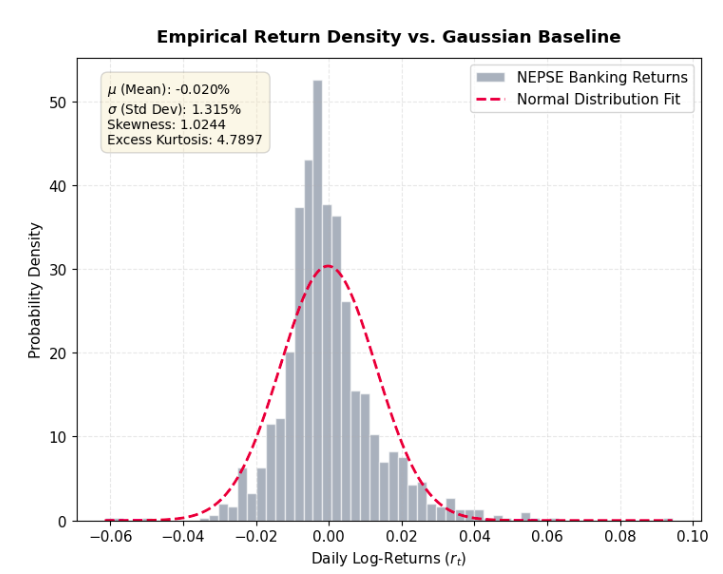
\includegraphics[width=\linewidth]{figures/emperical-vs-gaussian.png}
  \captionof{figure}{Empirical density vs.\ Gaussian: leptokurtic
    peak and fat tails \cite{cont2001empirical} (Fig.\ 2.1).}
\end{columns}
\end{frame}

\begin{frame}{Normal Q-Q Plot \& Volatility Clustering}
\begin{columns}[T]
\column{0.50\textwidth}
  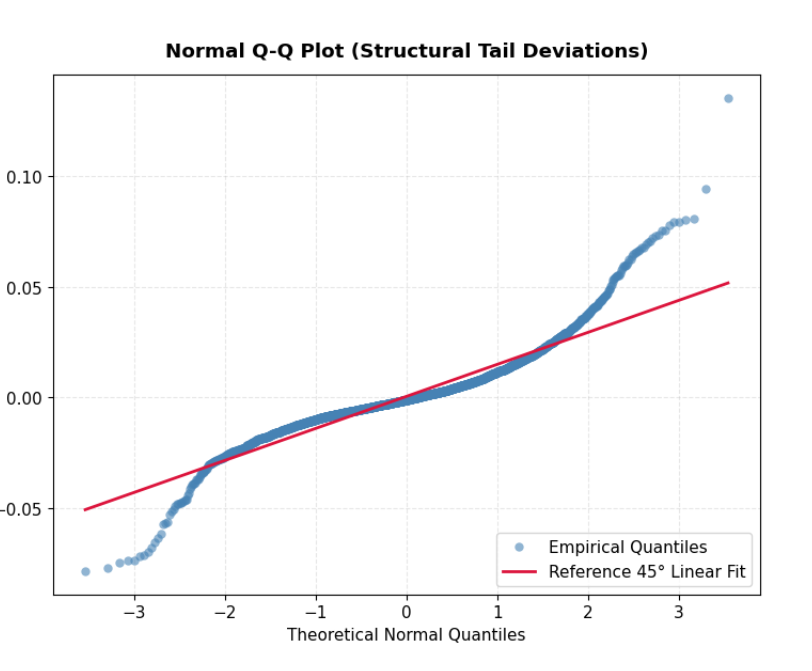
\includegraphics[width=\linewidth]{figures/normal-q-q.png}
  \captionof{figure}{Normal Q-Q plot: extreme quantiles lie far outside
    Gaussian confidence bands (Fig.\ 2.2).}
\column{0.50\textwidth}
  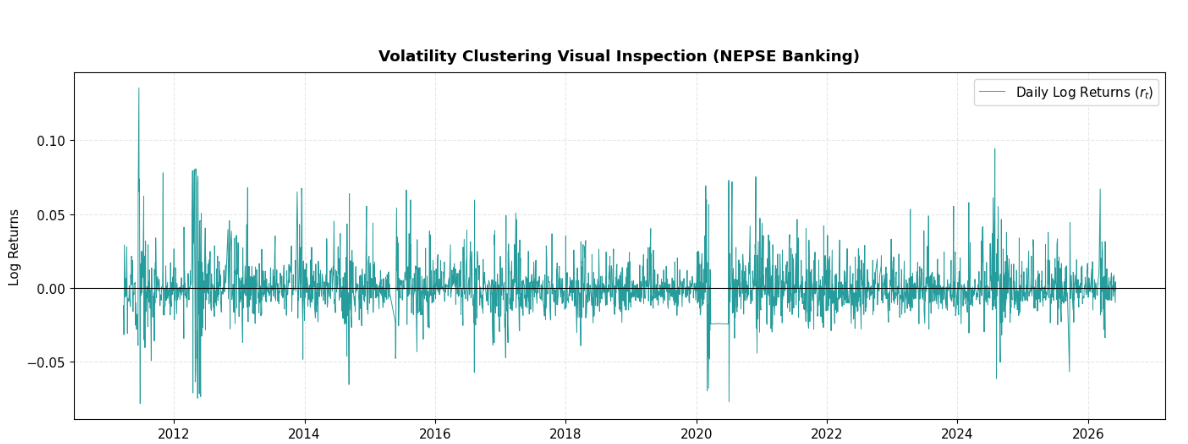
\includegraphics[width=\linewidth]{figures/volatility-clustering-visual-inspection.png}
  \captionof{figure}{Log-returns with 21-day rolling volatility corridor:
    alternating calm and turbulent episodes (Fig.\ 2.4).}
\end{columns}
\vspace{0.1cm}
\begin{itemize}
  \item Heavy tails motivate the \textbf{jump component} in the model.
  \item Volatility clustering motivates the \textbf{GARCH feedback} in $V_t$.
\end{itemize}
\end{frame}

\begin{frame}{Serial Dependence \& ARCH Effects}
\begin{columns}[T]
\column{0.58\textwidth}
  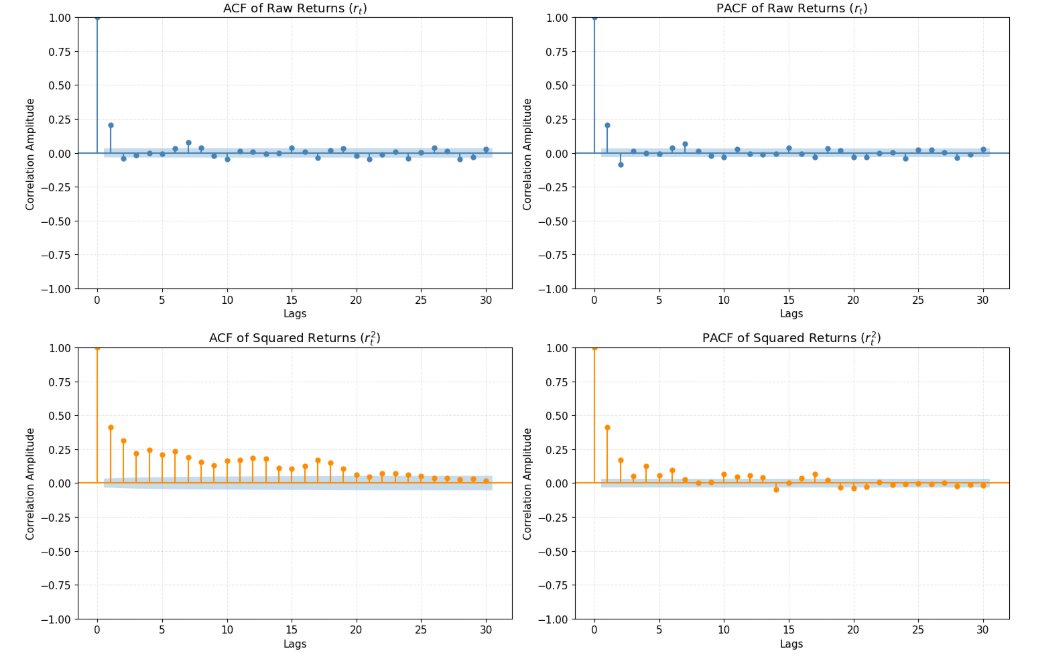
\includegraphics[width=\linewidth]{figures/acf-pacf.png}
  \captionof{figure}{ACF/PACF: raw (top) and squared returns (bottom) —
    hyperbolic decay in squared returns signals long-memory
    clustering \cite{engle1982autoregressive} (Fig.\ 2.3).}
\column{0.42\textwidth}
  {\small\begin{tabular}{l c}
    \toprule
    Test & $p$-value \\
    \midrule
    LB(10) raw & $<.001$ \\
    LB(20) raw & $<.001$ \\
    LB(10) sq. & $<.001$ \\
    LB(20) sq. & $<.001$ \\
    ARCH LM(10) & $<.001$ \\
    \midrule
    ADF & $<10^{-20}$ \\
    KPSS & $>0.1$ \\
    \bottomrule
  \end{tabular}}
  \vspace{0.15cm}
  \begin{itemize}\small
    \item Strong ARCH effects confirmed.
    \item \textbf{No leverage}: symmetric GARCH admissible.
    \item \textbf{Stationary} series (ADF rejects unit root;
          KPSS does not reject stationarity).
  \end{itemize}
\end{columns}
\end{frame}

\begin{frame}{Jump Detection \& Structural Break}
\begin{columns}[T]
\column{0.50\textwidth}
  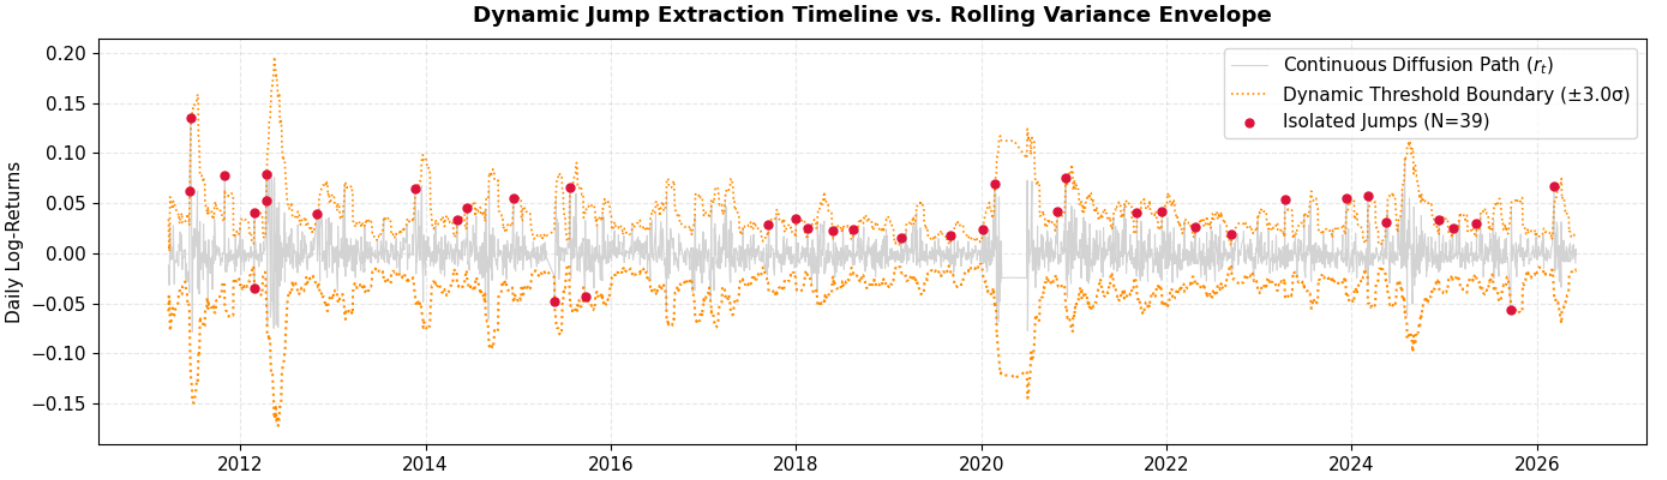
\includegraphics[width=\linewidth]{figures/dynamic-jump.png}
  \captionof{figure}{Dynamic $3\sigma$ filter (21-day rolling window):
    39 detected jumps, $1.12\%$ of trading days (Fig.\ 2.5).}
\column{0.50\textwidth}
  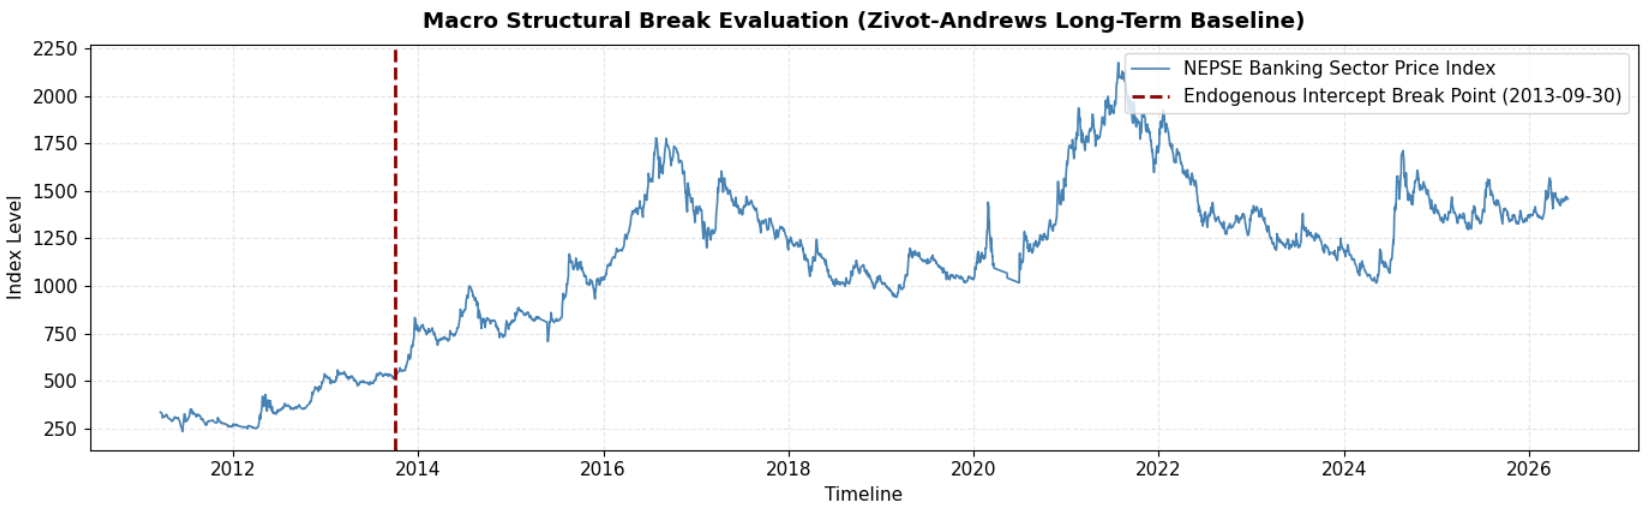
\includegraphics[width=\linewidth]{figures/breakdown.png}
  \captionof{figure}{Zivot--Andrews test: endogenous break at
    \textbf{30 Sep 2013} defines homogeneous post-break sample
    (Fig.\ 2.6).}
\end{columns}
\vspace{0.1cm}
\begin{columns}[T]
\column{0.50\textwidth}
  \begin{block}{Jump Statistics}
    $\lambda_{\mathrm{annual}}=2.83$ jumps/year;
    mean inter-arrival $=88.4$ days (median $75.5$ days).
  \end{block}
\column{0.50\textwidth}
  \begin{block}{Structural Break}
    ZA stat $=-3.17$ ($p=0.852$): no permanent break.
    Break date used to define a homogeneous estimation window.
  \end{block}
\end{columns}
\end{frame}

\begin{frame}{Empirical Chaos Diagnostics: Tail Index \& Long Memory}
\begin{columns}[T]
\column{0.50\textwidth}
  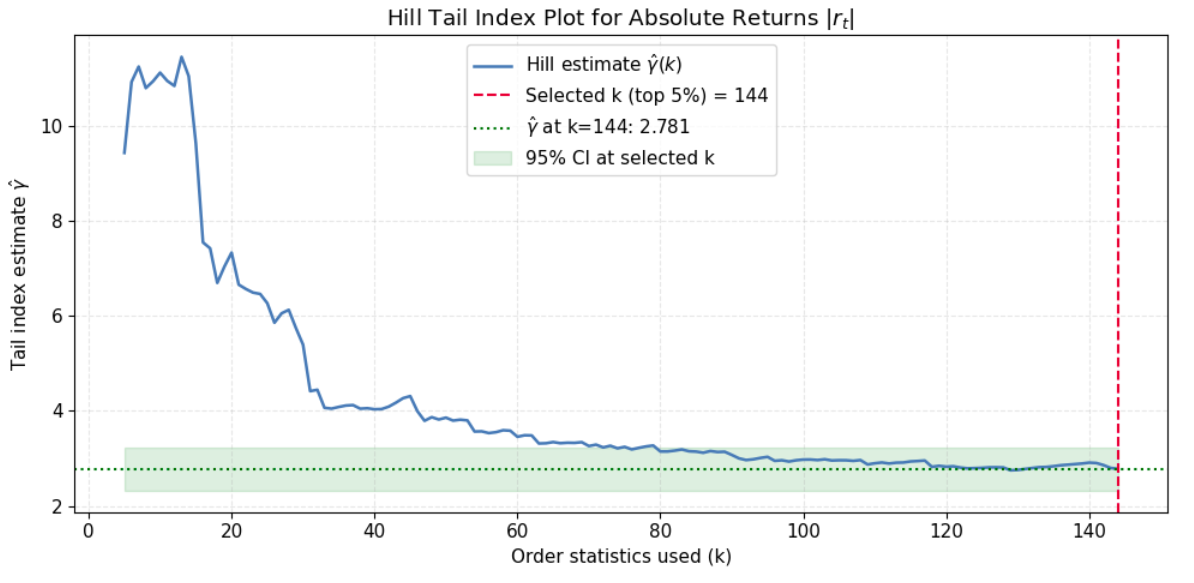
\includegraphics[width=\linewidth,height=0.48\textheight,keepaspectratio]{figures/hill-tail-index.png}
  \captionof{figure}{Hill tail-index $\hat{\gamma}$ vs.\ order statistics
    $k$; stabilises near $k\approx 140$ (5\% of sample) (Fig.\ 2.7).}
  \vspace{0.15cm}
  \begin{block}{Tail Index}\small
    $\hat{\gamma}=2.7805\pm 0.4542$ — finite variance
    ($\gamma>2$), power-law tails.
  \end{block}
\column{0.50\textwidth}
  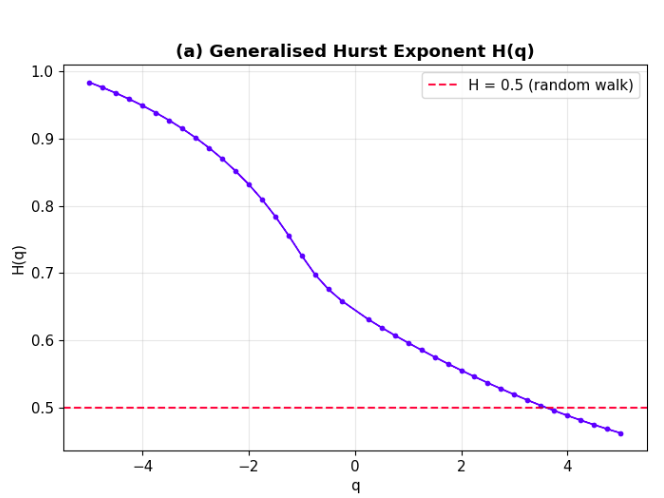
\includegraphics[width=\linewidth,height=0.48\textheight,keepaspectratio]{figures/hurst-exponent.png}
  \captionof{figure}{Generalised Hurst exponent $H(q)$; decreasing
    profile confirms multifractality \cite{peters1994fractal}
    (Fig.\ 2.8).}
  \vspace{0.15cm}
  \begin{block}{Long Memory}\small
    $H=0.7751>0.5$ — persistent dependence in $|r_t|$
    \cite{peters1994fractal}. Hyperbolic ACF decay.
  \end{block}
\end{columns}
\end{frame}

\begin{frame}{Empirical Chaos Diagnostics: Multifractality}
\begin{columns}[T]
\column{0.50\textwidth}
  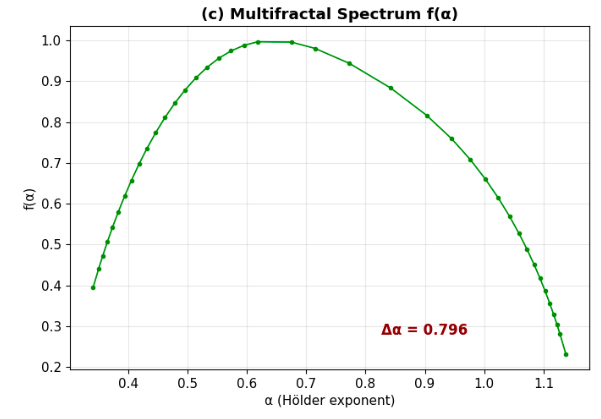
\includegraphics[width=\linewidth,height=0.48\textheight,keepaspectratio]{figures/multi-fractal.png}
  \captionof{figure}{Multifractal spectrum $f(\alpha)$ vs.\ Hölder
    exponent $\alpha$: broad parabolic shape (Fig.\ 2.9)
    \cite{calvet2002multifractality}.}
  \vspace{0.1cm}
  \begin{alertblock}{Multifractal Width}\small
    $\Delta\alpha = 0.7959$ — rich cascade structure consistent with
    \cite{mandelbrot2013fractals,calvet2002multifractality}.
  \end{alertblock}
\column{0.50\textwidth}
  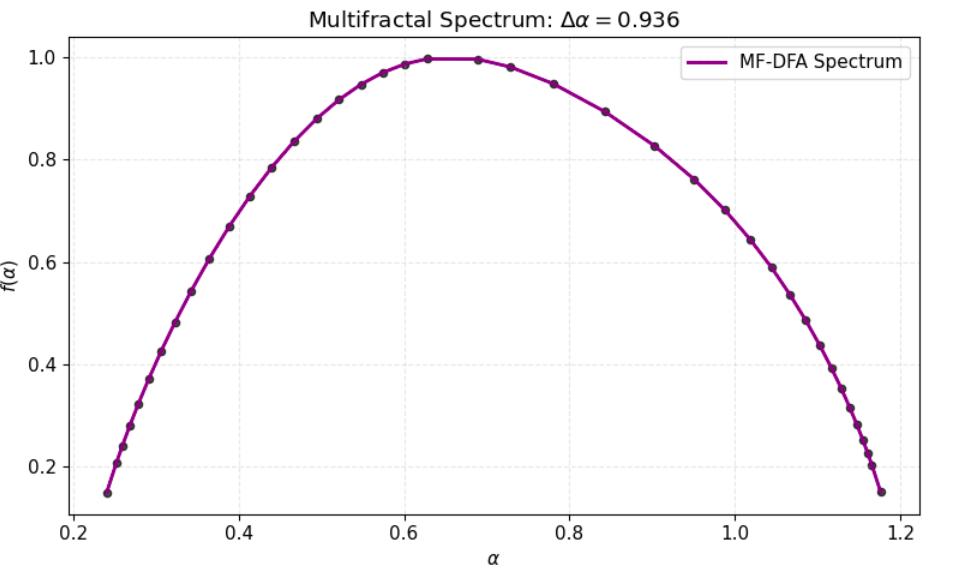
\includegraphics[width=\linewidth,height=0.48\textheight,keepaspectratio]{figures/mf-dfa-spectrum.png}
  \captionof{figure}{MF-DFA scaling: non-linear $H(q)$ across
    moment orders $q \in [-5,5]$
    \cite{calvet2002multifractality}.}
  \vspace{0.1cm}
  \begin{block}{Implication}\small
    Multiple scaling regimes confirm nonlinear, non-normal dynamics
    consistent with the COGARCH framework.
  \end{block}
\end{columns}
\end{frame}

% ================================================================
% CHAPTER 3 — COGARCH MODEL & ESTIMATION
% ================================================================
\section{COGARCH Model \& Estimation}

\begin{frame}{Model Specification (Kl\"uppelberg, Lindner \& Maller, 2004)}
\begin{columns}[T]
\column{0.55\textwidth}
  \textbf{Jump-Diffusion Price \& Variance SDEs \cite{kluppelberg2004continuous}:}
  \begin{align*}
    \frac{dS_t}{S_{t-}} &= \alpha\,dt + \sqrt{V_{t-}}\,dW_t
      + \bigl(e^{\sqrt{V_{t-}}Z}-1\bigr)dN_t,\\
    dV_t &= \kappa(\theta-V_{t-})\,dt + \phi\,V_{t-}\,Z^2\,dN_t,
  \end{align*}
  with $W_t$ Brownian motion, $N_t\sim\text{Poisson}(\lambda)$,
  $Z\sim\mathcal{N}(0,1)$ i.i.d.

  \medskip
  \textbf{Branching ratio:}
  \[
    B = \frac{\lambda\,\phi\,\mathbb{E}[Z^2]}{\kappa}
  \]
  $B\to 1^-$: near-critical self-excitation.
  $B<1$: stable mean-reverting volatility.
\column{0.45\textwidth}
  \begin{block}{GARCH(1,1) Discrete Approximation}
    \begin{align*}
      \omega &= \kappa\theta, \\
      \alpha_1 &= \phi\lambda, \\
      \beta_1 &= 1-\kappa.
    \end{align*}
    Persistence: $\alpha_1 + \beta_1 = 1 - \kappa + \phi\lambda$.
  \end{block}
  \vspace{0.2cm}
  \begin{block}{Key Symbols}
    $\kappa$: mean reversion; $\theta$: long-run variance;
    $\phi$: jump feedback; $\lambda$: jump intensity.
    See List of Symbols (thesis front matter).
  \end{block}
\end{columns}
\end{frame}

\begin{frame}{Method of Simulated Moments (MSM) \& Estimation Results}
\begin{columns}[T]
\column{0.50\textwidth}
  \textbf{MSM procedure \cite{kluppelberg2004continuous}:} minimise
  weighted squared distance between empirical and simulated moments:
  \begin{itemize}\small
    \item Mean, std.\ dev., skewness, excess kurtosis
    \item ACF of $|r_t|$ at lags 1 and 5
    \item Hill tail index (top 5\% of $|r_t|$)
  \end{itemize}
  Optimiser: \textbf{differential evolution}
  (10 paths per evaluation).

  \medskip
  {\small\begin{tabular}{l c}
    \toprule
    Parameter & Estimate \\
    \midrule
    $\kappa$ (annual) & $0.0729$ \\
    $\theta$ (annual var.) & $0.000213$ \\
    $\phi$ & $0.7100$ \\
    $\lambda$ (daily) & $0.0767$ \\
    $\lambda$ (annual) & $19.335$ \\
    \midrule
    \textbf{Branching ratio} $B$ & $\mathbf{0.7468}$ \\
    \bottomrule
  \end{tabular}}
\column{0.50\textwidth}
  \begin{alertblock}{Branching Ratio}
    \[
      B = \frac{0.0767 \times 0.7100}{0.0729} = 0.7468
    \]
    Below the near-critical window $[0.9,1)$ documented in
    developed markets \cite{hardiman2013critical}.
  \end{alertblock}
  \vspace{0.3cm}
  \begin{block}{GARCH(1,1) Persistence}
    $\alpha_1 = 0.0545$,\quad $\beta_1 = 0.9271$\\
    $\alpha_1 + \beta_1 = \mathbf{0.9815}$\\[4pt]
    Very high persistence confirms strong volatility clustering.
  \end{block}
\end{columns}
\end{frame}

% ================================================================
% CHAPTER 4 — CHAOS DIAGNOSTICS & MODEL VALIDATION
% ================================================================
\section{Chaos Diagnostics \& Model Validation}

\begin{frame}{Model-Implied vs.\ Empirical Diagnostics}
\begin{table}
\centering
\caption{Empirical vs.\ model-implied chaos diagnostics —
  synthetic path of 50,000 observations (Table 4.1 in thesis)}
\begin{tabular}{l c c c}
  \toprule
  Diagnostic & Empirical & Model-implied & Match? \\
  \midrule
  Tail index $\gamma$ (Hill, $|r_t|$) & $2.7805$ & $2.8928$ & \checkmark \\
  Hurst exponent $H$ (DFA, $|r_t|$)   & $0.7751$ & $0.8260$ & \checkmark \\
  Multifractal width $\Delta\alpha$    & $0.7959$ & $0.8096$ & \checkmark \\
  \bottomrule
\end{tabular}
\end{table}
\vspace{0.3cm}
The slight overestimation of $H$ and $\Delta\alpha$ is within sampling
variability.  The COGARCH captures tail heaviness, long memory, and
multifractal structure remarkably well.
\end{frame}

\begin{frame}{Chaotic Conditions Check \& Filtered Volatility}
\begin{columns}[T]
\column{0.50\textwidth}
  \begin{alertblock}{Theoretical Conditions \cite{kluppelberg2004continuous}}
    \begin{enumerate}[(i)]\small
      \item Near-critical: $B\in[0.9,1)$?
            \textbf{No} — $B=0.7468$ \quad $\times$
      \item Heavy tails: $\gamma\le 2$?
            \textbf{No} — $\gamma=2.78$ \quad $\times$
      \item Long memory: $H>0.5$?
            \textbf{Yes} — $H=0.775$ \quad \checkmark
      \item Multifractality: $\Delta\alpha>0.1$?
            \textbf{Yes} — $\Delta\alpha=0.796$ \quad \checkmark
    \end{enumerate}
  \end{alertblock}
  \vspace{0.2cm}
  Two of four conditions met.  NEPSE does \emph{not} exhibit the
  \textbf{full} chaotic regime, but long memory and multifractality
  \textbf{alone} justify the COGARCH for risk management.
\column{0.50\textwidth}
  \begin{block}{Why $B<0.9$? \cite{hardiman2013critical}}
    \begin{itemize}\small
      \item Lower liquidity in NEPSE than in developed markets.
      \item Fewer algorithmic / HFT participants.
      \item Smaller derivatives market — weaker self-exciting
            feedback loop.
    \end{itemize}
  \end{block}
  \vspace{0.2cm}
  \begin{block}{GARCH Filtered Volatility}
    Persistence $\alpha_1+\beta_1=0.9815$ confirms strong
    clustering.  Time-varying conditional variance detects more
    jump days than the simple rolling filter.
  \end{block}
\end{columns}
\end{frame}

% ================================================================
% CHAPTER 5 — RISK QUANTIFICATION
% ================================================================
\section{Risk Quantification}

\begin{frame}{Monte Carlo Simulation: Price Paths \& Return Distribution}
\begin{columns}[T]
\column{0.50\textwidth}
  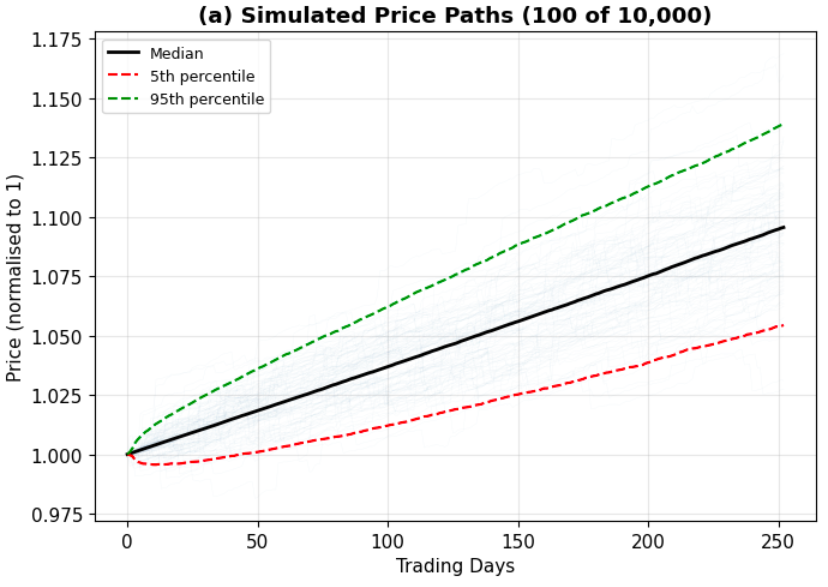
\includegraphics[width=\linewidth]{figures/simulated-paths.png}
  \captionof{figure}{100 of 10,000 COGARCH paths (252 days).
    Black: median; red: 5th pctile; green: 95th pctile.
    Fan shape reflects volatility persistence and jump risk
    (Fig.\ 5.1).}
\column{0.50\textwidth}
  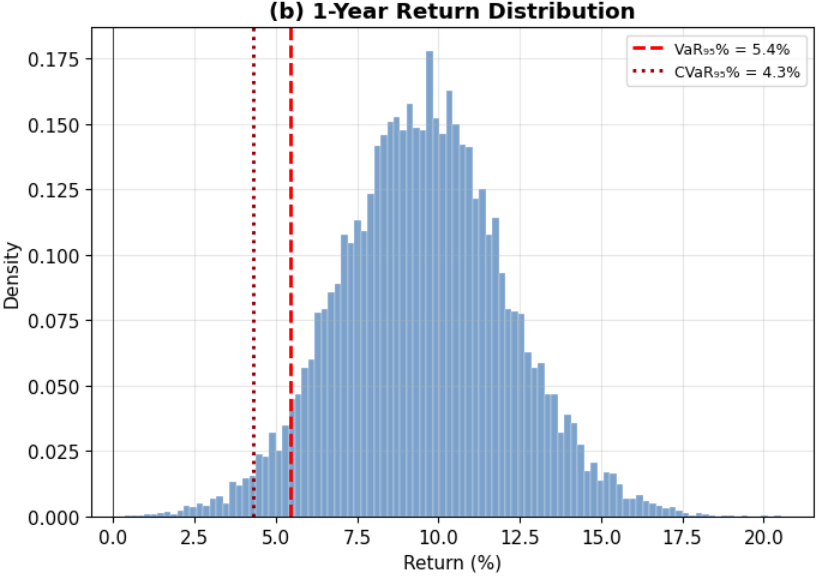
\includegraphics[width=\linewidth]{figures/one-year-return.png}
  \captionof{figure}{Terminal 1-year simple return distribution:
    right-skewed, mode near $+10\%$, small heavy left tail
    (Fig.\ 5.2).}
\end{columns}
\end{frame}

\begin{frame}{Risk Measures \& Gaussian Comparison}
\begin{columns}[T]
\column{0.50\textwidth}
  \textbf{One-year Risk Measures} (10,000 COGARCH paths,
  Table 5.1 in thesis)\\[4pt]
  {\small\begin{tabular}{l c}
    \toprule
    Measure & Value \\
    \midrule
    VaR$_{95\%}$ & $-1.7\%$ \\
    VaR$_{99\%}$ & $-6.2\%$ \\
    CVaR$_{95\%}$ (Exp.\ Shortfall) & $-4.4\%$ \\
    CVaR$_{99\%}$ & $-8.3\%$ \\
    P(negative annual return) & $8.4\%$ \\
    P(drawdown $>30\%$) & $0.0\%$ \\
    \bottomrule
  \end{tabular}}
\column{0.50\textwidth}
  \begin{alertblock}{Gaussian Benchmark (Ch.\ 5, Sec.\ 2)}
    Annualised vol $\approx 24.3\%$.\\
    Gaussian VaR$_{95\%}\approx -40\%$ —
    \textbf{grossly over-conservative}.\\
    Gaussian VaR$_{99\%}\approx -56.5\%$.
  \end{alertblock}
  \vspace{0.2cm}
  \begin{block}{COGARCH Advantage}
    \begin{itemize}\small
      \item Mean reversion + jump dynamics $\Rightarrow$
            \textbf{realistic, not inflated} tail estimates.
      \item Daily VaR$_{95\%}\approx -0.11\%$: operationally
            usable.
      \item CVaR $\gg$ VaR: tail losses are severe when they
            occur — critical for capital adequacy rules.
    \end{itemize}
  \end{block}
\end{columns}
\end{frame}

% ================================================================
% CHAPTER 6 — DISCUSSION
% ================================================================
\section{Discussion}

\begin{frame}{Discussion: Interpretation of Results}
\begin{columns}[T]
\column{0.50\textwidth}
  \begin{itemize}
    \item All EDA evidence (density, Q-Q, ACF, multifractal spectrum)
          points to \textbf{nonlinear, non-equilibrium dynamics} in the
          NEPSE banking sector.
    \item Estimated COGARCH parameters reproduce empirical $\gamma$,
          $H$, $\Delta\alpha$ within sampling variability.
    \item $B=0.7468$ — self-exciting feedback \textbf{weaker} than in
          US/UK markets \cite{hardiman2013critical}: low liquidity,
          few HFT participants, small derivatives market.
    \item $\gamma\approx 2.78$ implies \textbf{finite variance}
          ($\gamma>2$) — less extreme than crisis-era developed markets,
          yet close to the critical value $\gamma=2$.
  \end{itemize}
\column{0.50\textwidth}
  \begin{block}{For Investors \& Risk Managers}
    \begin{itemize}\small
      \item COGARCH VaR/CVaR far more accurate than Gaussian models.
      \item Annual jump intensity $=19.3$/year: frequent volatility
            spikes relevant for position sizing and stop-loss rules.
      \item 8.4\% probability of negative annual return: useful
            benchmark for strategic asset allocation.
    \end{itemize}
  \end{block}
  \vspace{0.2cm}
  \begin{block}{For Regulators}
    \begin{itemize}\small
      \item Use COGARCH to stress-test under simulated jump scenarios.
      \item Branching ratio $B$ as an early-warning metric for
            systemic criticality in the banking sector.
    \end{itemize}
  \end{block}
\end{columns}
\end{frame}

\begin{frame}{Discussion: Limitations \& Future Work (Ch.\ 6, Sec.\ 3)}
\begin{enumerate}
  \item \textbf{Data frequency}: Daily data misses intraday jumps;
        5-min or 1-min data would sharpen $\lambda$ and $\phi$ estimates.
  \item \textbf{Constant jump intensity}: Poisson $\lambda$ is
        restrictive; a \alert{Hawkes self-exciting process}
        \cite{hardiman2013critical} would capture jump clustering.
  \item \textbf{Parameter stability}: No permanent break found (ZA test),
        but a \alert{regime-switching COGARCH} via rolling-window MSM
        could reveal time-varying dynamics.
  \item \textbf{Model comparison}: Future work should compare COGARCH
        with GARCH-jump and EGARCH using AIC/BIC and out-of-sample
        forecasting.
  \item \textbf{Multivariate extension}: Banking sector index is an
        aggregate; systemic risk across individual banks requires a
        multivariate COGARCH.
\end{enumerate}
\end{frame}

% ================================================================
% CONCLUSION
% ================================================================
\section{Conclusion}

\begin{frame}{Conclusion}
\begin{itemize}
  \item \textbf{EDA} (Ch.\ 2): NEPSE returns exhibit non-normality,
        volatility clustering \cite{bollerslev1986generalized},
        long memory ($H=0.775$) \cite{peters1994fractal},
        and multifractality ($\Delta\alpha=0.796$)
        \cite{calvet2002multifractality}.
  \item \textbf{COGARCH estimation} (Ch.\ 3): MSM yields $B=0.7468$,
        persistence $=0.9815$, $\lambda_{\rm annual}=19.3$
        \cite{kluppelberg2004continuous}.
  \item \textbf{Chaos validation} (Ch.\ 4): model reproduces empirical
        $\gamma$, $H$, $\Delta\alpha$; 2/4 criticality conditions met.
  \item \textbf{Risk quantification} (Ch.\ 5):
        VaR$_{95\%}=-1.7\%$, CVaR$_{95\%}=-4.4\%$,
        VaR$_{99\%}=-6.2\%$ (one-year) vs.\ Gaussian
        over-estimate of $\approx -40\%$.
  \item Provides a \textbf{replicable blueprint} for testing nonlinear
        criticality in any emerging equity market
        \cite{worldbank2020nepal,gajurel2021volatility}.
\end{itemize}
\end{frame}

% ================================================================
% THANK YOU
% ================================================================
\begin{frame}[plain]{}
  \begin{center}
    \vspace{0.8cm}
    
\includegraphics[height=2.2cm]{photos/kulogo.jpg}\\[0.7cm]
    {\Large\textbf{Thank You for Your Attention!}}\\[0.5cm]
    {\normalsize\textbf{Tek Raj Pant}}\\[0.15cm]
    {\small Department of Mathematics, School of Science\\
    Kathmandu University, Dhulikhel, Nepal}\\[0.4cm]
    {\small\textit{References and questions follow.}}
  \end{center}
\end{frame}

% ================================================================
% REFERENCES
% ================================================================
\begin{frame}[allowframebreaks]{References}
  \nocite{*}
  \bibliographystyle{unsrt}
  \bibliography{references}
\end{frame}

% ================================================================
% QUESTIONS
% ================================================================
\begin{frame}[plain]{}
  \begin{center}
    \vspace{0.6cm}
    {\scalebox{4}{\textbf{?}}}\\[0.6cm]
    {\LARGE\textbf{Questions?}}\\[0.4cm]
    {\normalsize Please feel free to ask.}\\[0.3cm]
    {\small Tek Raj Pant $\mid$ Kathmandu University}
  \end{center}
\end{frame}

\end{document}